\documentclass{l4proj}
\usepackage{tikz}
\usepackage{etoolbox}
\usepackage{listings-rust}

\usetikzlibrary{calc,arrows}

\begin{document}
\makeatletter
% make numeric styles use name format
\patchcmd{\NAT@test}{\else \NAT@nm}{\else \NAT@nmfmt{\NAT@nm}}{}{}

% define \citepos just like \citet
\DeclareRobustCommand\citepos
{\begingroup
    \let\NAT@nmfmt\NAT@posfmt
    \NAT@swafalse\let\NAT@ctype\z@\NAT@partrue
    \@ifstar{\NAT@fulltrue\NAT@citetp}{\NAT@fullfalse\NAT@citetp}}

\let\NAT@orig@nmfmt\NAT@nmfmt
\def\NAT@posfmt#1{
    \StrRemoveBraces{#1}[\NAT@temp]
    \IfEndWith{\NAT@temp}{s}
    {\NAT@orig@nmfmt{#1'}}
    {\NAT@orig@nmfmt{#1's}}}

\makeatother

\title{Improving MQTT at the transport layer using QUIC}
\author{Ivan Nikitin}
\date{\today}

\maketitle

\begin{abstract}
    New advances in networked systems and programming languages are set to succeed existing industry standards.
    In the transport layer space, QUIC - a is set to succeed the TCP/TLS stack and is advantageous for performance and security by leveraging improved features such as a simpler, secure handshake, and streams.
    While in the programming languages space, Rust, a new systems programming language, uses a strong type system to guarantee memory-safety and deadlock-freedom, while still being performant.
    In this work we analyse the feasibility of using a Rust based QUIC implementation as the basis for secure communication in IoT devices.
    To do so, in this work we develop $MQuicTT$ - a Rust based MQTT implementation using QUIC at the transport layer.
    We compare the performance of the resulting solution with existing MQTT implementations in various use cases and analyse the hardware resources needed to deploy it.
    We find that the performance of the implementation is on par with the baseline.
    Finally, we discuss the binary size of the implementation and the possible methods to generally reduce Rust binary sizes for IoT network firmware using QUIC.
\end{abstract}

\def\consentname {Ivan Nikitin} % your full name
\def\consentdate {25 March 2022} % the date you agree
\educationalconsent


\tableofcontents

\chapter{Introduction}

% reset page numbering. Don't remove this!
\pagenumbering{arabic} 

The Internet of Things (IoT) is rapidly becoming the most prominent form of computation, with the number of IoT devices projected to surpass 75 billion by 2025~\citep{statista_number_2016}.
IoT devices range from daily consumer gadgets such as wearables to sensors that are used in smart factories.
The central theme of these devices is network connectivity.
Network firmware installed on these devices has to be performant enough to send and receive massive amounts of data. 
Hence, the need for efficient, lightweight network firmware often means that manufacturers of these devices forego security for performance~\cite{ling_iot_2018}.
Therefore, the mass use of devices that are manufactured without security in mind creates a situation where many devices that are critical to infrastructure become vulnerable to cyber attacks, as seen in the 2015 attack on the Ukraine power grid~\citep{Liang2017}.
However, we can not just employ the usual methods to secure firmware on these devices due to the presented constraints in terms of their physical size, power consumption needs and available hardware resources.
Hence, there is a need to develop protocols for secure, performant communication for IoT devices.

MQTT~\citep{oasis_mqtt_2014} is a popular message-passing network protocol designed to be lightweight for the IoT use case.
While certain protocols have been developed to specifically act as data transfer protocols for IoT devices, MQTT remains the most widely used.
MQTT's design ensures that the protocol's implementations have a small code footprint and take up minimal network bandwidth.
Significantly, MQTT relies on a transport layer protocol to send data and ensure secure communication.
The standard in current MQTT implementations is to use TLS to provide secure data transfer.
As we present in this work, this adds overhead, which means that the advantages of MQTT are negated if we need secure communication.

There have recently been several developments in systems software that aim to succeed in existing industry standards.
QUIC~\citep{iyengar_quic_2021}, a new transport layer network protocol initially designed at Google, is set to succeed TCP with a number of improvements.
QUIC boasts advantages in both secure communication and performance by eliminating several overheads of TCP such as head of line blocking and requiring a much simpler handshake to establish a secure connection.
In addition to this, the Rust programming language is a memory-safe systems programming language that aims to succeed C.
Rust is secure by design due to its type-system and still provides the needed efficiency due to its region-based memory management approach adding no real overhead.

Hence, to take advantage of the developments made in the transport protocol and programming languages spaces, we must analyse if a Rust implementation of QUIC can be a viable alternative to existing widely-deployed implementations.

To do so, we introduce MQuicTT - a QUIC port of an MQTT library in the Rust programming language, discuss the design choices made during its development, analyse its performance and discuss the challenges IoT presents for network protocols.
We show that $MQuicTT$ is as performant as the baseline chosen TCP MQTT implementation in our testing scenarios.
We further analyse the steps needed to create protocols for hardware constrained devices and present an analysis for the methodology of lowering the overhead of a QUIC stack.
Finally, we analyse the libraries and features that contribute to the binary size of Rust implementations.

\section{Dissertation Outline}

The rest of this dissertation is structured as follows:
\begin{itemize}
    \item Chapter~\ref{chap:back} provides a background on the recent developments in the transport layer network protocol space, IoT and the Rust programming language.
    \item Chapter~\ref{chap:reqs} presents the requirements that were set to answer our research questions and the design of the implementation of $MQuicTT$ and its ecosystem.
    \item Chapter~\ref{chap:impl} details the implementation of $MQuicTT$ and $QuicSocket$ - an intermediate QUIC API that we have developed. This chapter also presents a discussion of the choices made during implementation and the difficulties that we circumvented.
    \item Chapter~\ref{chapter:eval} details the experiment design and analysis of $MQuicTT$ and provides a discussion of results.
    \item Finally, Chapter~\ref{chap:conclusion} concludes and summarises important results and discusses avenues for future work.
\end{itemize}
\chapter{Background}

\section{The evolution of the transport layer}

This section presents a background of the network protocols at the transport layer, starting from the currently dominant standards and ending with new advancements in the field.
We also consider how to provide secure communication at the transport layer using encryption.

First described by~\citet{cerf_protocol_1974}, the Transmission Control Protocol (TCP) has been the primary protocol of the Internet suite since its initial implementation.
TCP provides a \textit{reliable} and \textit{ordered} delivery of bytes, ensuring that data is not lost, altered or duplicated and delivered in the same order as intended by the sender.
TCP achieves this by assigning a sequence number to each transmitted packet and requiring an \textit{acknowledgement} (commonly referred to as ACK) from the receiving side.
If an ACK is not received, the data is re-transmitted.
TCP can also use the sequence numbers to order packets in the order intended by the sender on the receiving side.

As TCP is a connection-based protocol, connection establishment must occur before any data can be transmitted.
The receiving side (the server) must bind to and listen on a network port, and the sender (the client) must initiate the connection using the process of a \textit{three-way handshake} as shown in Figure \ref{fig:tcp}.
In the first step of the handshake, the client sends a segment with a \textit{synchronise sequence number} (SYN) that indicates the start of the communication and the sequence number that the segment starts with.
The server responds with an acknowledgement - ACK, and the sequence number it will start its segment with - SYN.
Hence, we refer to this step as the SYN-ACK.
In the third and final step, the client must acknowledge the response.
At this point, TCP establishes the connection and can transfer data on it.

\begin{figure}[ht]
    \begin{center}
        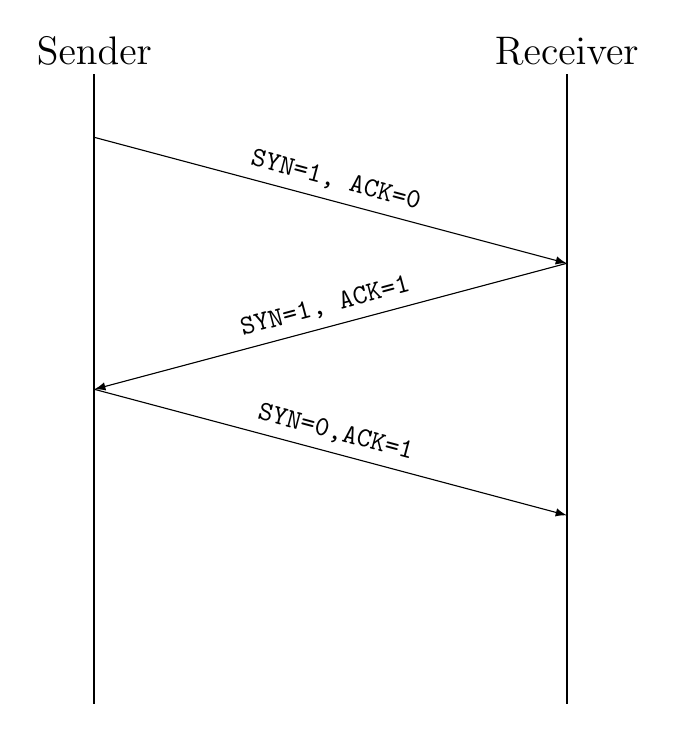
\begin{tikzpicture}[>=latex]
            \coordinate (A) at (2,8);
            \coordinate (B) at (2,0);
            \coordinate (C) at (8,8);
            \coordinate (D) at (8,0);
            \draw[thick] (A)--(B) (C)--(D);
            \draw (A) node[above]{\Large Sender};
            \draw (C) node[above]{\Large Receiver};

            \coordinate (E) at ($(A)!.1!(B)$);
            \draw (E) node[left]{\begin{tabular}{r}
                \end{tabular}};

            \coordinate (F) at ($(C)!.3!(D)$);
            \draw (F) node[right]{\begin{tabular}{l}
                \end{tabular}};
            \draw[->] (E) -- (F) node[midway,sloped,above]{\verb$SYN=1, ACK=0$};

            \coordinate (G) at ($(A)!.5!(B)$);
            \draw (G) node[left]{};
            \draw[->] (F) -- (G) node[midway,sloped,above]{\verb$SYN=1, ACK=1$};

            \coordinate (H) at ($(A)!.5!(B)$);
            \draw (H) node[right]{};

            \coordinate (I) at ($(C)!.7!(D)$);
            \draw (I) node[left]{};
            \draw[->] (H) -- (I) node[midway,sloped,above]{\verb$SYN=0,ACK=1$};
        \end{tikzpicture}
        \caption{The TCP handshake needed for connection establishment. The values of the SYN and ACK fields being set indicate the kind of segment sent. For example, for the SYN-ACK stage both the SYN and ACK fields are set.}
        \label{fig:tcp}
    \end{center}
\end{figure}

In order to achieve \textit{secure communication}, TLS~\citep{rescorla_transport_2018} is often used in the TCP stack.
In order to do this, a separate TLS handshake has to occur in order to specify the version of TLS to use, decide on the cypher suites, authenticate the server via its public key and certificate authority's signature, and generate a session key that the protocol uses for symmetric encryption during communication.
In the TLS handshake, the first step is for the client to send a $ClientHello$ message that specifies the highest version of TLS that the client supports, a list of suggested cypher suites, compression methods and a random number.
The server responds with a $ServerHello$ message containing the selected TLS version, cypher suite, compression method, and random number.
The server then sends its certificate and $ServerKeyExchange$ message along with the $ServerHelloDone$ message indicating that it has completed its part of the negotiation process.
The client will respond with the $ClientKeyExchange$ message (CKE), which may contain a public key depending on the chosen cypher suite.
Following this, the client sends a $ChangeCipherSpec$ message indicating that communication from this point is authenticated and encrypted.
The client combines this message with a client finished message.
The server responds with the same message, establishing the TLS connection.

Due to the establishment of communication and properties guaranteed by TCP, this process lengthens communication latency.
Hence, in use-cases where reliability and connection state is not required, the User Datagram Protocol (UDP)~\citep{j_postel_1980} is preferred.
UDP uses a connectionless communication model with a minimal number of implementation semantics.
The only mechanisms provided by UDP are port numbers and checksums in order to ensure data integrity.
UDP is preferable for real-time systems as using TCP would cause overhead to latency and retransmission of packets that the application no longer needs.

While TCP and UDP have been the dominant standards of the internet since its creation, QUIC is a relatively new general-purpose transport layer protocol. QUIC was first designed by~\citet{jim_roskind_2012} at Google as part of the Chromium web engine and standardised by the IETF in 2021~\citep{iyengar_quic_2021}.
It aims to improve upon, and eventually make obsolete, TCP by using the concept of multiplexing over a UDP connection.
Multiplexing is a method of combining several signals or channels of communication over one shared medium.
QUIC makes use of multiplexing by facilitating data exchange on the UDP connection through the concept of \textit{streams}.
Streams are an ordered byte-stream abstraction used by the application to send data of any length.
Any number of QUIC streams, unidirectional or bidirectional, can be created by either side during the connection.
Hence, QUIC allows an arbitrary number of streams to send arbitrary amounts of data on a single UDP connection, subject to the constraints imposed by flow control.

By doing so, QUIC also achieves other performance benefits.
For example, QUIC lifts congestion control algorithms from the kernel space to the userspace.
Hence, congestion control algorithms can evolve without being tied down to kernel level semantics and constraints.

\begin{figure}[t]
    \begin{center}
        \begin{subfigure}[b]{0.45\textwidth}
            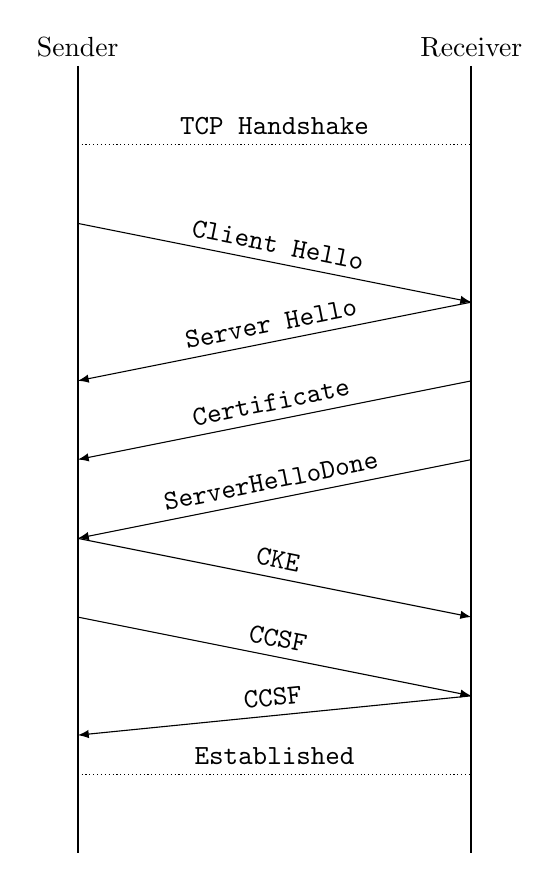
\begin{tikzpicture}[>=latex]
                \coordinate (A) at (2,10);
                \coordinate (B) at (2,0);
                \coordinate (C) at (7,10);
                \coordinate (D) at (7,0);
                \draw[thick] (A)--(B) (C)--(D);
                \draw (A) node[above]{Sender};
                \draw (C) node[above]{Receiver};

                \coordinate (H) at ($(A)!.1!(B)$);
                \draw (H) node[right]{};

                \coordinate (I) at ($(C)!.1!(D)$);
                \draw (I) node[left]{};
                \draw[densely dotted] (H) -- (I) node[midway,sloped,above]{\verb$TCP Handshake$};

                \coordinate (H) at ($(A)!.2!(B)$);
                \draw (H) node[right]{};

                \coordinate (I) at ($(C)!.3!(D)$);
                \draw (I) node[left]{};
                \draw[->] (H) -- (I) node[midway,sloped,above]{\verb$Client Hello$};

                \coordinate (H) at ($(C)!.3!(D)$);
                \draw (H) node[right]{};

                \coordinate (I) at ($(A)!.4!(B)$);
                \draw (I) node[left]{};
                \draw[->] (H) -- (I) node[midway,sloped,above]{\verb$Server Hello$};

                \coordinate (H) at ($(C)!.4!(D)$);
                \draw (H) node[right]{};

                \coordinate (I) at ($(A)!.5!(B)$);
                \draw (I) node[left]{};
                \draw[->] (H) -- (I) node[midway,sloped,above]{\verb$Certificate$};

                \coordinate (H) at ($(C)!.5!(D)$);
                \draw (H) node[right]{};

                \coordinate (I) at ($(A)!.6!(B)$);
                \draw (I) node[left]{};
                \draw[->] (H) -- (I) node[midway,sloped,above]{\verb$ServerHelloDone$};

                \coordinate (H) at ($(A)!.6!(B)$);
                \draw (H) node[right]{};

                \coordinate (I) at ($(C)!.7!(D)$);
                \draw (I) node[left]{};
                \draw[->] (H) -- (I) node[midway,sloped,above]{\verb$CKE$};

                \coordinate (H) at ($(A)!.7!(B)$);
                \draw (H) node[right]{};

                \coordinate (I) at ($(C)!.8!(D)$);
                \draw (I) node[left]{};
                \draw[->] (H) -- (I) node[midway,sloped,above]{\verb$CCSF$};

                \coordinate (H) at ($(C)!.8!(D)$);
                \draw (H) node[right]{};

                \coordinate (I) at ($(A)!.85!(B)$);
                \draw (I) node[left]{};
                \draw[->] (H) -- (I) node[midway,sloped,above]{\verb$CCSF$};

                \coordinate (H) at ($(A)!.9!(B)$);
                \draw (H) node[right]{};

                \coordinate (I) at ($(C)!.9!(D)$);
                \draw (I) node[left]{};
                \draw[densely dotted] (H) -- (I) node[midway,sloped,above]{\verb$Established$};
            \end{tikzpicture}
            \caption{TCP/TLS}
            \label{fig:handshakes:tls}
        \end{subfigure}
        \begin{subfigure}[b]{0.45\textwidth}
            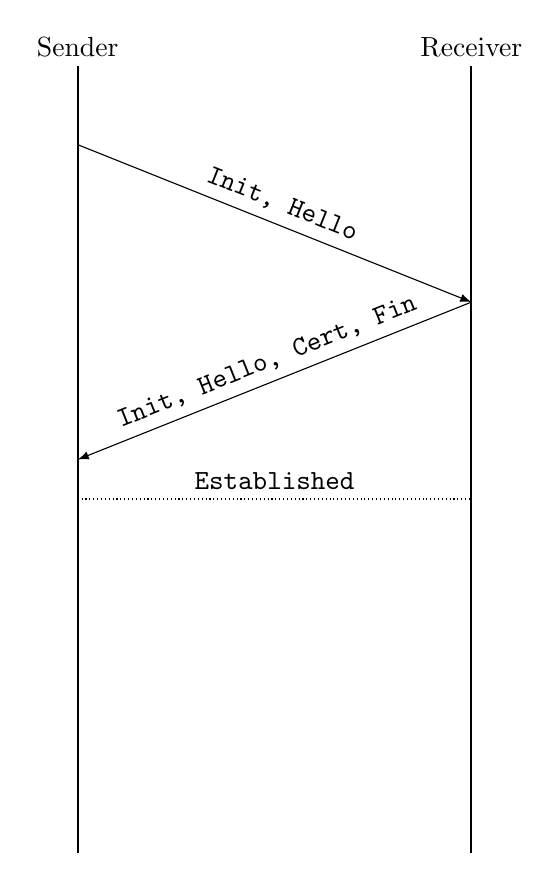
\begin{tikzpicture}[>=latex]
                \coordinate (A) at (2,10);
                \coordinate (B) at (2,0);
                \coordinate (C) at (7,10);
                \coordinate (D) at (7,0);
                \draw[thick] (A)--(B) (C)--(D);
                \draw (A) node[above]{Sender};
                \draw (C) node[above]{Receiver};

                \coordinate (E) at ($(A)!.1!(B)$);
                \draw (E) node[left]{\begin{tabular}{r}
                    \end{tabular}};

                \coordinate (F) at ($(C)!.3!(D)$);
                \draw (F) node[right]{\begin{tabular}{l}
                    \end{tabular}};
                \draw[->] (E) -- (F) node[midway,sloped,above]{\verb$Init, Hello$};

                \coordinate (G) at ($(A)!.5!(B)$);
                \draw (G) node[left]{};
                \draw[->] (F) -- (G) node[midway,sloped,above]{\verb$Init, Hello, Cert, Fin$};

                \coordinate (H) at ($(A)!.55!(B)$);
                \draw (H) node[right]{};

                \coordinate (I) at ($(C)!.55!(D)$);
                \draw (I) node[left]{};
                \draw[densely dotted] (H) -- (I) node[midway,sloped,above]{\verb$Established$};
            \end{tikzpicture}
            \caption{QUIC}
            \label{fig:handshakes:quic}
        \end{subfigure}
        \caption{Handshakes required to establish secure data transmission in the TCP/TLS stack \subref{fig:handshakes:tls} and the QUIC stack \subref{fig:handshakes:quic}. In the case of TCP/TLS, we can see that the handshake is substantially more complex and that the TLS handshake requires the full TCP handshake before it can proceed. In both cases, these handshakes can be made quicker. In the case of TLS, version 1.3 allows for one less round trip before data can be sent, and in the case of QUIC 0-RTT, connection re-establishment may be used in some cases, allowing to send data in the first packet.}
        \label{fig:handshakes_comparison}
    \end{center}
\end{figure}

Compared to TCP/TLS, QUIC combines the transport and cryptographic handshakes to minimise the time needed for connection establishment; Figure~\ref{fig:handshakes_comparison} shows a comparison of the handshakes.
QUIC still uses TLS functionality to secure communication as described by~\citet{thomson_using_2021} unless the developer specifies a different cryptographic protocol; however, this is done differently to TCP.
The initial QUIC handshake keeps the same handshake messages as TLS; however, it uses its framing format, replacing the TLS record layer.
This use ensures that the connection is always authenticated and encrypted, unlike TLS, where the initial handshake is vulnerable.
The combination also means that QUIC typically starts sending data after one round-trip, achieving security by default and lower latency.

\section{The Internet of Things}
\section{Rust programming language}

Rust is a modern systems programming language created at Mozilla designed to be highly safe and performant.
It is a systems language that aims to maintain the performance that we expect from languages like C while also using a unique \textit{ownership} system to maintain memory safety.
Instead of garbage collection, Rust opts for a system managed through the resource acquisition is initialisation (RAII) principle~\citep{rust_raii_2021}.
All values have a unique owner, and their scope is tied to this owner.
Hence, by design, Rust does not allow dangling pointers, null pointers, and data races as the compiler will not allow for a programmer to compile unsafe code without circumventing it using the $unsafe$ keyword.

For example, consider the program written in C in Listing~\ref{lst:C} compared to a similar application in Rust in Listing~\ref{lst:Rust}.
The C program demonstrates a use after free bug.
The pointer is freed and then used in the print statement, resulting in undefined behaviour.
While this example is relatively trivial, these bugs are often tough to debug in a more extensive, more complex system, leading to security vulnerabilities.
This issue does not only exist in codebases and organisations with low resources; at the BlueHat security conference, Microsoft researcher~\cite{miller_msrc-security-research2019_02_2019} presented that Microsoft targets roughly 70\% of their yearly patches at fixing memory safety bugs.
On the other hand, the analogous Rust code will not compile due to the ownership system, mitigating this issue altogether.

\begin{lstlisting}[language=C, caption={An example of a use after free in C code. This is an incorrect use of dynamic memory management, however it compiles. In large, complex code bases, missing bugs such as these often happens and can cause exploitable security issues.}, label=lst:C]
    void bar() {
        int *ptr = (Point *) malloc(sizeof(int));
        free (ptr);
        printf("%d", *ptr); // obvious use after free, however this will compile
    }
\end{lstlisting}

\begin{lstlisting}[language=Rust, float, caption={A similar application in Rust will not compile due to the safety guaranteed by the ownership system. A borrow occurs when $example\_ref$ is assigned to point to $new\_example$, however the ownership system recognises that the borrowed value does not live long enough.}, label=lst:Rust]
    fn bar() {
        let example = String::from("Example");
        let mut example_ref = &example;
        {
            let new_example = String::from("New Example");
            example_ref = &new_example;
        }
        println!("our string is {}", &example_ref); // causes a compiler error in Rust: error `new_example` does not live long enough
    }
\end{lstlisting}

When it comes to networked systems in the IoT space, Rust is a natural application due to its focus on concurrency and safe systems programming.
Firstly, a memory-safe language may circumvent security-related bugs in IoT firmware and the supporting network stacks.
As previously discussed, getting the firmware correct on the first try is essential in IoT due to the difficulty of providing updates.
However, assessing the performance of Rust implementations of the QUIC stack is vital to solidifying Rust as a performant systems programming language for hardware constrained devices.
If the binary sizes produced by the Rust implementations are larger than their C equivalents or if the code is not as performant, then the memory safety guarantees may not matter for IoT developers.

\chapter{Foundational implementations}\label{chap:libs}

\subsection{QUIC} \label{section:quic_impl}

We now compare the existing implementations of the QUIC protocol in the context of usability for IoT devices and present the reasoning behind our choice of QUIC library.
We have considered the mainstream implementations in the C, C++, Rust and Go programming languages as these are the languages that can be considered systems languages and would thus be the most widely used ones for IoT devices.
In addition to this, we did not consider implementations paired with a browser web engine as these would be impossible to use on hardware constrained devices.
Hence, we did not include notable implementations such as the QUIC implementation of the chromium web engine~\citep{chromium_quic_2021} and $Neqo$~\citep{mozilla_neqo_2022}.

Importantly, to analyse the performance of underlying QUIC implementations, we have transferred the same file using each implementation several times and have taken the average time to do so.
We repeated this while altering parameters as described in Section~\ref{chap:net_sim}.
The differences in transfer time were negligible and have hence not been presented as part of the comparison of libraries.
Hence, we compare QUIC implementations in terms of their TLS use, programming language and the binary size produced by their client and server implementations.

First, we consider the general landscape of available QUIC implementations to contextualise the ones developed in Rust.
Table~\ref{tab:quics} demonstrates the analysed QUIC implementations.
In order to find the size of the binary, we have used the Linux $ls$ utility.
In the case of the $mvfst$ implementation, we have taken further steps due to the reported binary size being far too large.
Therefore, we had to remove the C++ debug symbols that were causing the binary size to be over 300 MiB.
We have identified the following main methods by which QUIC implementations incorporate TLS:

\begin{itemize}
    \item Use of an external library - the implementation uses an external TLS API either by using a package manager in the case of Rust or by relying on an installed implementation in the case of C and C++.
    \item Use of own implementation - the implementation packages its implementation of the TLS protocol alongside QUIC.
\end{itemize}

This different use of TLS presented a challenge in calculating the binary size of the QUIC servers and clients.

\begin{table}[ht]
    \caption{The identified QUIC implementations and their binary size footprint. The footprint has been split into a client and server footprint using a minimal reproducible example for each. We used each implementation to create an example client and server capable of sending and receiving QUIC packets and analysed the binary size. Where provided, we compared this to the given examples to ensure as little implementation bias as possible. However, this is still not a perfect estimate, and some variance due to implementation details may be present.}\label{tab:quics}
    %\tt 
    \rowcolors{2}{}{gray!3}
    \begin{tabular}{@{}lllll@{}}
        \toprule
        \textbf{Implementation} & \textbf{PL}   & \textbf{Footprint (client) (MiB)} & \textbf{Footprint (server) (MiB)} & \textbf{TLS method} \\
        ngtcp2                  & \texttt{C}    & \texttt{3.4}                      & \texttt{4.3}                      & \texttt{External}   \\
        picoquic                & \texttt{C}    & \texttt{3.2}                      & \texttt{3.9}                      & \texttt{External}   \\
        msquic                  & \texttt{C}    & \texttt{3.2}                      & \texttt{4.1}                      & \texttt{External}   \\
        quic-go                 & \texttt{Go}   & \texttt{8.7}                      & \texttt{9.9}                      & \texttt{External}   \\
        Quinn                   & \texttt{Rust} & \texttt{9.1}                      & \texttt{9.5}                      & \texttt{External}   \\
        Quiche                  & \texttt{Rust} & \texttt{7.8}                      & \texttt{7.0}                      & \texttt{Own}        \\
        mvfst                   & \texttt{C++}  & \texttt{11.1}                     & \texttt{12.0}                     & \texttt{Own}        \\
        \bottomrule
    \end{tabular}
\end{table}

Specifically, in each case, we have considered the external dependencies that a developer will have to install to run the QUIC implementation on a device.
Hence, in the case of C implementations that require an external TLS library, such as OpenSSL, to be installed and linked on the system, we have opted to add the binary size produced by OpenSSL to the size of the QUIC binaries.
Additionally, in the case of $picoquic$, we have added the size of the $picotls$ dependency on top of the size of OpenSSL.

\begin{figure}[ht]
    \centering
    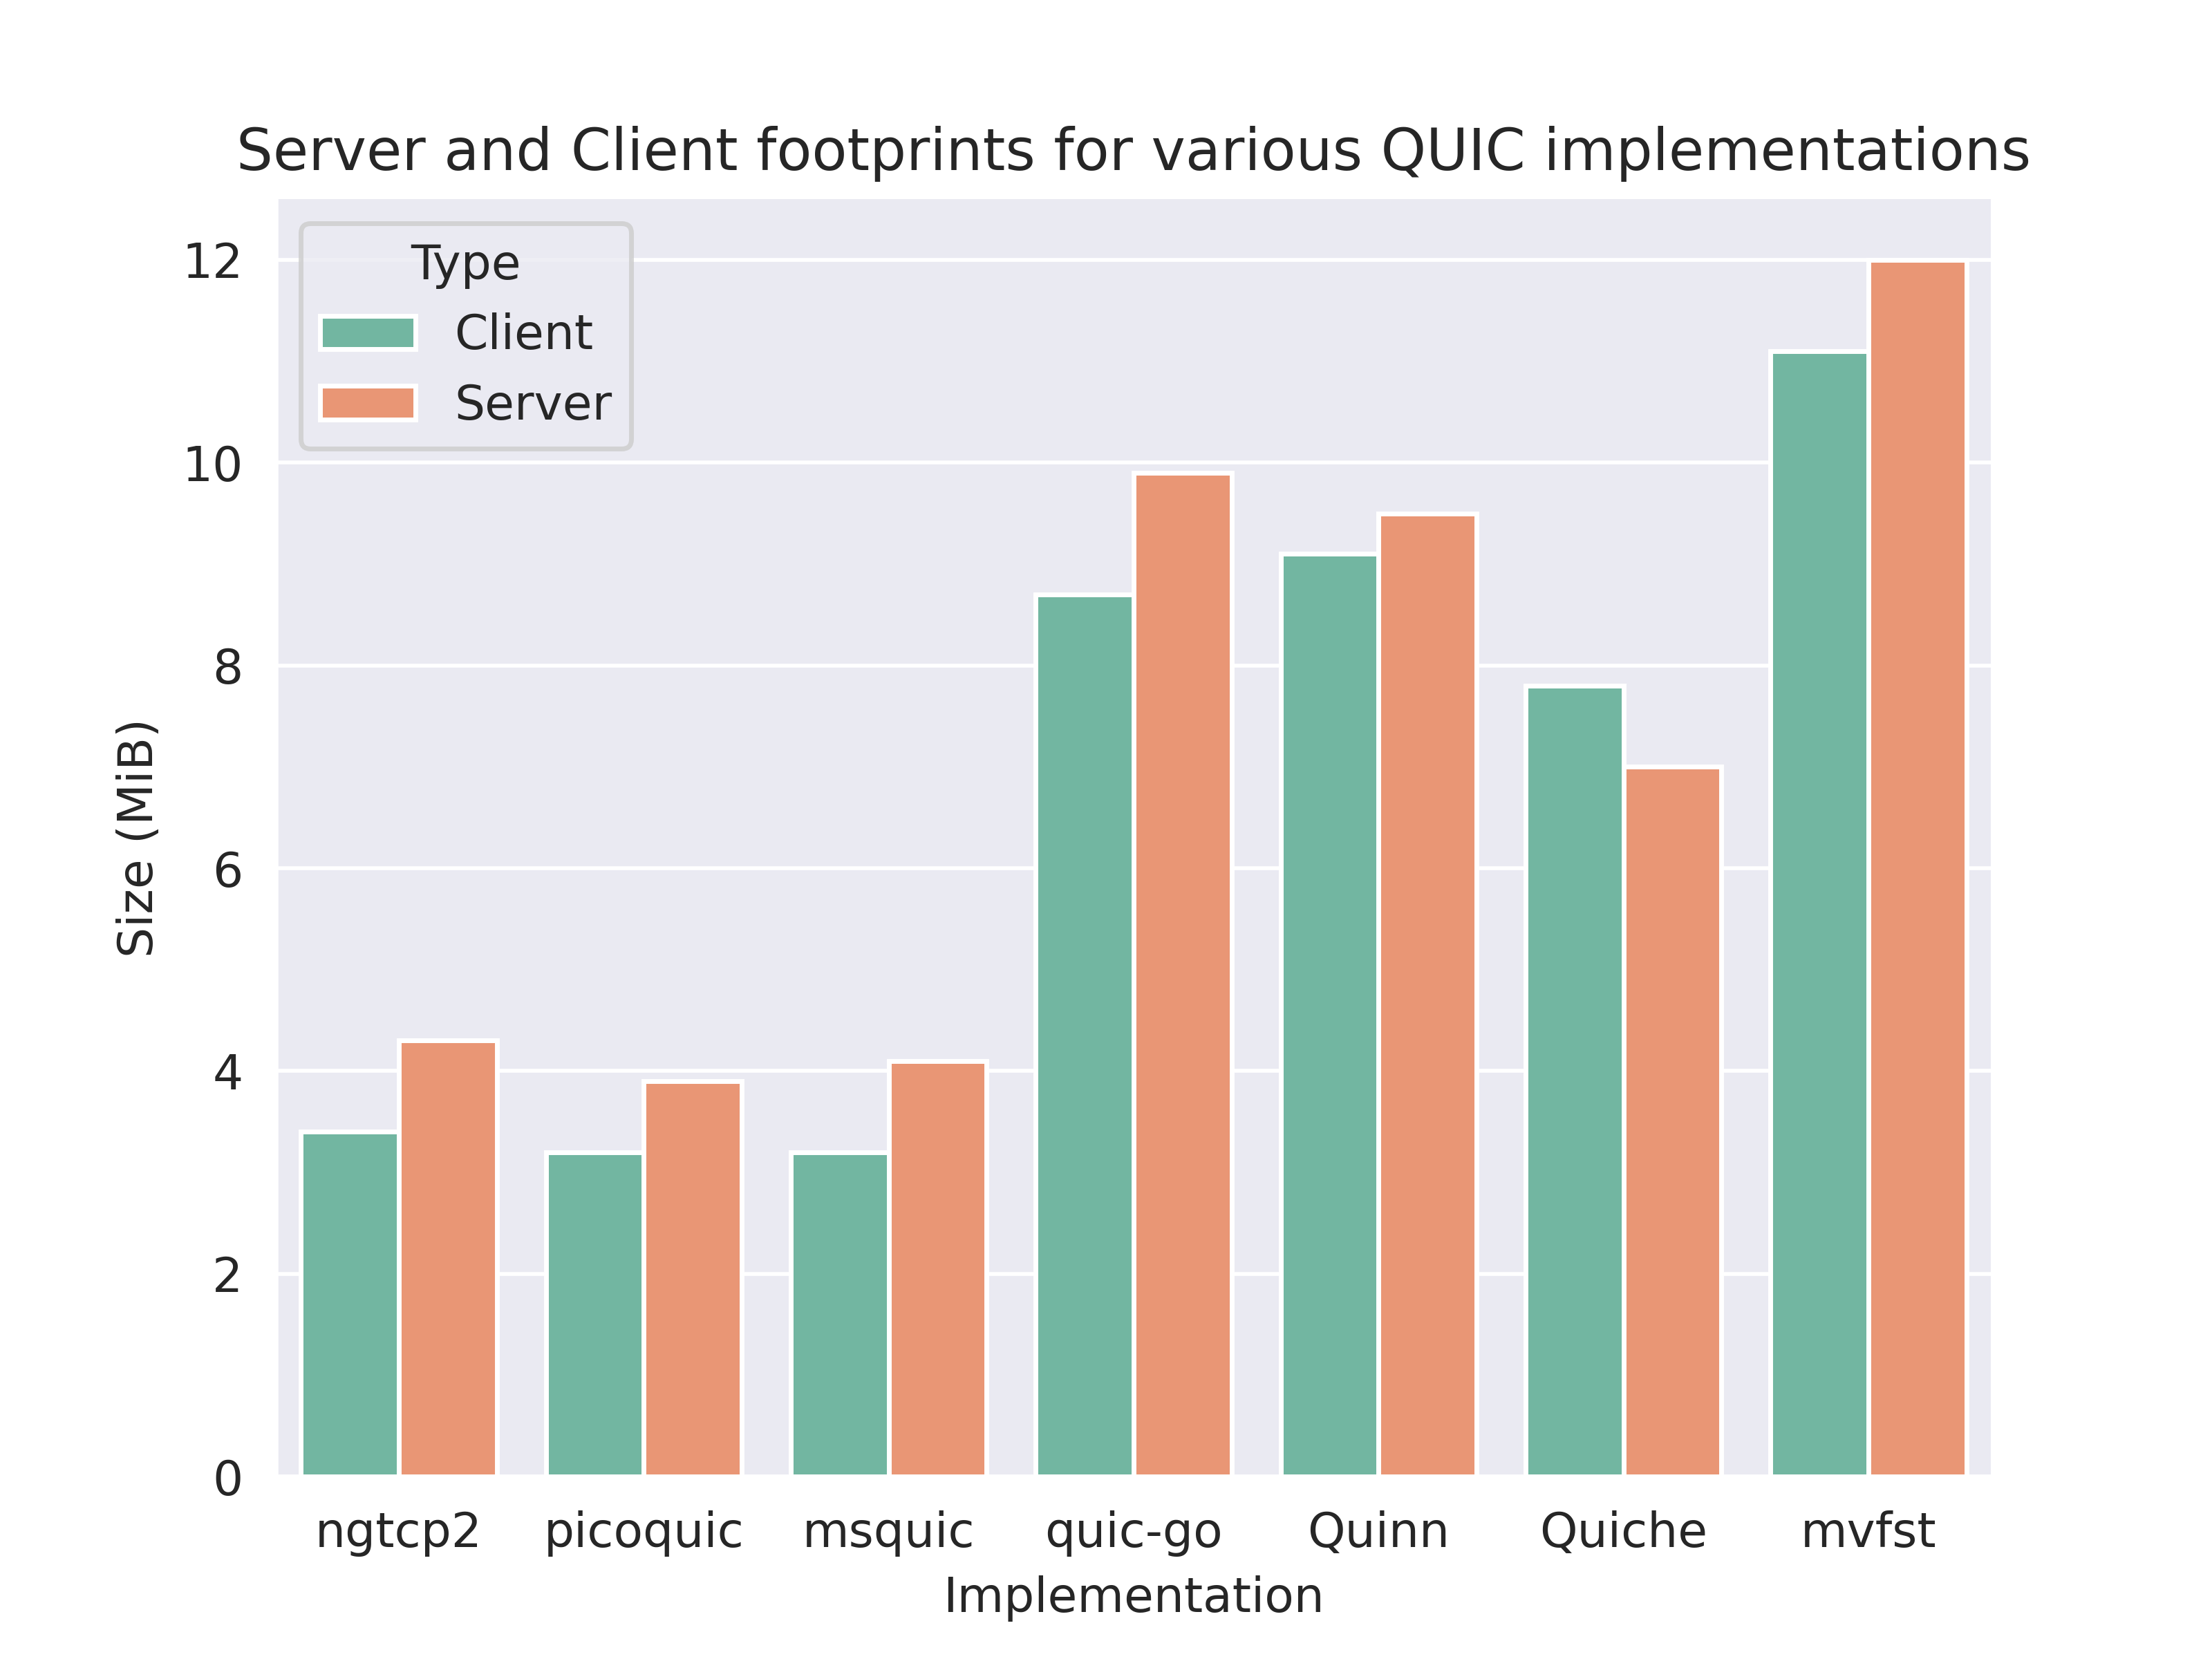
\includegraphics[width=1\linewidth]{images/quic_impls.png}
    \caption{The sizes of the client and server footprints for the selected QUIC implementations. Notable, only Quiche produced a server binary with a smaller size than its corresponding client binary. It is hard to estimate the error margin for the data as this depends on implementation details in the example client and servers.}
    \label{fig:quic_impls}
\end{figure}

Figure~\ref{fig:quic_impls} further visualises the comparison of binary sizes between the various implementations.
This is an important aspect due to the aforementioned hardware constraints.
Notably, we can see that five out of the seven analysed implementations opt to use an external TLS library or engine.
Out of these five, all C implementations supported OpenSSL, with the Go and Rust implementations opting to use a TLS library.
In the case of $quic-go$, this was the $crypto/tls$ package, and in the case of Rust, $rustls$.
We can also see that the Rust implementations are not drastically different in binary footprint size.

Notably, although Go is described as memory safe, it does not opt for compile-time memory safety and instead uses the panic model.
The panic model is another advantage of Rust compared to languages such as Go, as Rust provides these guarantees using a robust type system.
Between the two Rust implementations - Quinn and Quiche, we chose Quinn due to issues with the Quiche library.
On the other hand, Quiche opts to make the user create a $mio$ event loop, which interfered with the $tokio$ runtime environment used in our chosen MQTT implementation discussed in the next section.
In addition to this, we found that the Quinn API is easier to work with when creating the intermediate library discussed in Chapter~\ref{chapter:quic_socket}; for example, Quinn handles the QUIC handshake in the library and does not require the developer to create an event loop.

\section{MQTT}\label{section:mqtt_impls}

Compared to QUIC, the choice of MQTT implementation was substantially simpler.
The criteria for MQTT implementation were that it was developed in Rust, implemented both a client and a broker, had widespread use and adhered to MQTT version 5.0.
Based on the above criteria we identified two possible implementations:\citepos{eclipse_eclipse_2018} $paho$ and $rumqtt$~\citep{bytebeam_rumqtt_2020}.
We opted to use $rumqtt$ at it is a native Rust implementation, whereas $paho$ provides a rust binding to an underlying C implementation.
We chose to evaluate a fully Rust native MQTT/QUIC stack as this provides an opportunity for a valuable comparison to mainstream C implementations.
Other available implementations supported only one side of the MQTT protocol or only supported version 3.1.1.

$Rumqtt$ provides to components for an MQTT application - $rumqttc$ and $rumqttd$.
The former can be used to create an MQTT client, and the latter a broker.
However, the code base for these is somewhat similar, easing the incorporation of QUIC.
Both components provide an interface for supporting asynchronous communication using a $tokio$ runtime, which fits nicely into our choice of QUIC implementation as $Quinn$ requires a $tokio$ environment.
By default, $rumqtt$ uses TCP as its transport layer protocol and TLS through $rustls$.
All underlying implementation assumptions remain equal because this is the same library as $Quinn$ uses.

\section{QuicSocket}\label{chapter:quic_socket}

This section will present $QuicSocket$~\footnote{QuicSocket - \url{https://github.com/Apolexian/QuicSocket}} - the intermediate wrapper API that we developed using $Quinn$ to facilitate establishing a QUIC connection, control streams, and send and receive data.

$QuicSocket$ provides two main types to communicate with $Quinn$ - a $QuicServer$ and a $QuicClient$, and a trait that both of these implement - $QuicSocket$.
The $QuicSocket$ trait defines three function: $new$, $send$ and $recieve$. 
When initialised using the $new$ function, the server and the client attempt to open a QUIC connection.
In the case of the server, it binds to a given port and starts listening for a connection request.
The client binds to a random available port and attempts to connect to a provided URL.
Additionally, in the $new$ function, the server generates a new TLS certificate or reads it from a specified path.
The client's $new$ function must be supplied with the corresponding certificate's path.
If either certificate is not present, the server will reject the connection attempt.
Once a connection has been opened, data transfer can happen.

\begin{lstlisting}[language=Rust, caption={The $send$ function that the $QuicClient$ and $QuicServer$ use for sending data. Data transfer is facilitated by opening a bidirectional stream on the pre-existing connection.}, label=lst:quicsocket_send]
    async fn send(&mut self, payload: Vec<u8>) -> Result<()> {
        let (mut send, _) = self
            .connection
            .open_bi()
            .await
            .map_err(|e| anyhow!("failed to open stream: {}", e))
            .unwrap();
        send.write_all(&payload)
            .await
            .map_err(|e| anyhow!("failed to send request: {}", e))?;
        send.finish()
            .await
            .map_err(|e| anyhow!("failed to shutdown stream: {}", e))?;
        Ok(())
    }
\end{lstlisting}

In order to send data, either side can use the $send$ function demonstrated in Listing~\ref{lst:quicsocket_send}.
We first open a bidirectional stream and then write the provided payload.
Once the client completes writing the payload, it shuts down the stream.
On the other side, the receive function in Listing~\ref{lst:quicsocket_recv} processes the next available QUIC stream and reads the data on it into a supplied buffer.
It then returns the number of bytes written to the buffer.
Hence, to use $QuicSocket$, we must either provide or generate TLS certificates, open a QUIC connection and then use the send and receive functions.
The developed API is analogous to how a TCP socket sends and receives data.
An alternative approach that we considered was to make the $recv$ function return the value that the client or server read from the stream.
However, this approach does not integrate well into any protocol implementation due to the general preference for the buffer pattern.

\begin{lstlisting}[language=Rust, float, caption={The $recv$ function that the $QuicClient$ and $QuicServer$ use for sending data.}, label=lst:quicsocket_recv]
    async fn recv(&mut self, buf: &mut [u8]) -> Result<usize> {
        let (_, mut recv) = self.bi_streams.next().await.unwrap().unwrap();
        let len = recv
            .read(buf)
            .await
            .map_err(|e| anyhow!("failed to read response: {}", e))?;
        Ok(len.unwrap())
    }
\end{lstlisting}

Error handling is handled via the $anyhow$ package throughout the library for idiomatic error handling.
In addition to this, we wrap return values in Rust's $Result$ construct.
Hence, all errors are idiomatically mapped wherever a failure can occur.

An important design choice that we have made when developing $QuicSocket$ is using QUIC streams.
Every call to send and receive in the current implementation creates a bidirectional stream.
An alternate choice was to open a stream at the start of the connection and use it until the connection closes.
However, the latter approach runs into issues when it comes to reading from the stream.
All data was read on one call to receive, which unnaturally coalesced MQTT packets.

Notably, all operations happen asynchronously.
However, as of the implementation time, the Rust standard library does not support asynchronous traits.
The workaround to this issue is using the $async-trait$ crate. 
An unfortunate drawback of using this crate is that every function call results in a heap allocation due to the crate's implementation semantics.
The extra heap allocations do not usually present an issue; however, in the case of hardware constrained devices, this may lead to a bottleneck depending on the usage of the library.
The reasons for not supporting asynchronous traits in Rust are somewhat complex.
For one, an asynchronous function in Rust returns an $impl Future$, meaning that an asynchronous trait would have to support returning $impl Trait$, which it does not.
However, the $async-trait$ crate instead returns a $dyn Future$, the Rust implementation of dynamic dispatch, resulting in a heap allocation but allowing it to be used inside of traits.
We will not further discuss the other reasons for this crate's existence; however,~\cite{matsakis_baby_2019} created a comprehensive analysis of this issue.
Once Rust incorporates asynchronous traits into the language, the heap allocation issue will be resolved, resulting in this problem no longer existing for hardware constrained devices.

\section{MQuicTT} \label{chap:port}

This section describes how we used $QuicSocket$ to create a QUIC port of $rumqtt$, the design decisions that we have taken, and possible alternate approaches.

As previously mentioned, $rumqtt$ provides two APIs: $rumqttc$ for creating MQTT clients and $rumqttd$ for creating brokers.
Hence, each of these APIs relies on an underlying TCP implementation to transmit data.
A configuration file is also required for $rumqtdd$ that specifies various parameters such as paths to TLS keys and the ports that MQTT will operate on.
Additionally, $rumqtt$ implements its own layer of TLS to ensure secure communication on top of the TLS layer provided by the underlying transport protocol.

To create $MQuicTT$, we have taken steps that can broadly be summarised in two phases: altering the default TLS code and changing the underlying transport protocol from TCP to QUIC.

As we are working in the domain of hardware constrained devices, providing multiple layers of encryption would be excessive, even for the goal of secure communication.
We can afford for only the transport layer to handle encryption.
Hence, the first step that we have taken is to remove all TLS functionality from both $rumqttd$ and $rumqttc$.

After this, we identified that both APIs have a central interface that controls network communication.
In the case of $rumqttc$ this is the $network$ struct inside $framed.rs$~\footnote{framed.rs - \url{https://github.com/bytebeamio/rumqtt/blob/master/rumqttc/src/framed.rs}} and in the case of $rumqttd$ it is the $network$ struct inside $network.rs$~\footnote{network.rs - \url{https://github.com/bytebeamio/rumqtt/blob/master/rumqttd/src/network.rs}}.
Both of these interfaces use a $tcpstream$ to send and receive data.
The $tcpstream$ is opened when the struct is initialised and closed when the MQTT connection ends.
As TCP is a stateful protocol, minimal connection handling occurs after opening the initial stream.

\begin{lstlisting}[language=Rust, caption={An example of initialising an $MQuicTT$ client. The QUIC connection is established by initialising a $QuicClient$ and the resulting client is passed as an MQTT option.}, label=lst:MQuicTT:client]
    #[tokio::main(worker_threads = 1)]
    async fn main() {
        ...
        let quic_client = QuicClient::new(None).await;
        let mut mqttoptions = MqttOptions::new("test-1", ip, 1883, addr, quic_client);
        mqttoptions.set_connection_timeout(10);
        mqttoptions.set_keep_alive(5);
    
        let (client, mut eventloop) = AsyncClient::new(mqttoptions, 100);
        task::spawn(async move {
            requests(client).await;
        });
    }
\end{lstlisting}

As we have modelled $QuicSocket$ to have an API that closely resembles a typical $tcpstream$ API, the challenge of this stage of the port was managing QUIC streams and the state of connection.
Due to UDP, the protocol that underlyes QUIC, being stateless, we have handled the connection differently in brokers and clients.

The connection request is sent before an MQTT client object is initialised in the client's case.
Upon successful connection, the programmer must pass the connection to the initialisation function of the client.
This means that a single QUIC connection underpins the client's entire MQTT connection, and streams are used for packets.
Hence, when the client wishes to close the MQTT connection, it also closes the underlying QUIC connection.
In order to do this we have modified the parameters needed to create an $rumqtt$ MQTT client.
An example of the initialisation of a QUIC connection and MQTT client using our implementation is demonstrated in Listing~\ref{lst:MQuicTT:client}.

In the case of a broker, we must wait for a client to send a connection request.
Hence, we may initialise the broker and wait for a QUIC connection, only allowing data transfer when any connection is established.
This also means that the broker does not need to track which connection comes from which client.

\begin{lstlisting}[language=Rust, caption={An example of initialising an MQuicTT broker. We can see that no operations with $QuicSocket$ are required for this initialisation as all QUIC operations are handled internally.}, label=lst:MQuicTT:broker]
    fn main() {
        pretty_env_logger::init();
        let config: Config = confy::load_path("rumqttd.conf").unwrap();
        let mut broker = Broker::new(config);

        let mut tx = broker.link("localclient").unwrap();
        thread::spawn(move || {
            broker.start().unwrap();
        });
        ...
    }

\end{lstlisting}

Hence, as we can see in Listing~\ref{lst:MQuicTT:broker}, the programmer is not required to use any $QuicSocket$ code when creating an $MQuicTT$ broker.

We considered an alternate approach to refactoring the $rumqtt$ codebase to consolidate all network code into a shared internal package.
This would mean that the API for creating a client and broker would be identical and perhaps more ergonomic.
However, we decided not to go with this approach because $rumqttc$ and $rumqttd$ would no longer be disjoint, independent components.
With the chosen approach, it is possible to use different underlying transport protocols for either side, which allows for flexibility in implementation.

Another avenue of discussion stems from $rumqtt$ having two different client implementations: a synchronous client and an asynchronous client.
In either case, a $tokio$ eventloop is used to handle events.
As $QuicSocket$ requires an asynchronous environment, the natural choice was to use the asynchronous client.
It could, however, be possible to handle asynchronous events more efficiently by tying the QUIC eventloop to the MQTT eventloop as in the approach described by~\cite{kumar_implementation_2019}.
In our case, we leave the comparison between these two approaches as an avenue for future work.

\section{Network performance experiment design} \label{chap:net_sim}

We now discuss the analysis methodology for the performance portion of the implementation evaluation.
That is, this section focuses on evaluating MQuicTT against the base $rumqtt$ implementation.

The critical consideration for this design is the scenarios in which IoT devices are used.
When evaluating the network performance of the implementations, we considered two options: using real IoT devices or using a network simulation tool.
Due to technical limitations that came with using real devices, such as not being able to access the router of our network, we opted for simulation.
In this section, we will discuss how we used Mininet~\citep{lantz_mininet_2021}, a realistic virtual network, in our evaluation.

Mininet is a tool that network developers and researchers can use to create software-defined networks (SNDs) using the $OpenFlow$ standard.

\begin{figure}[ht]
    \centering
    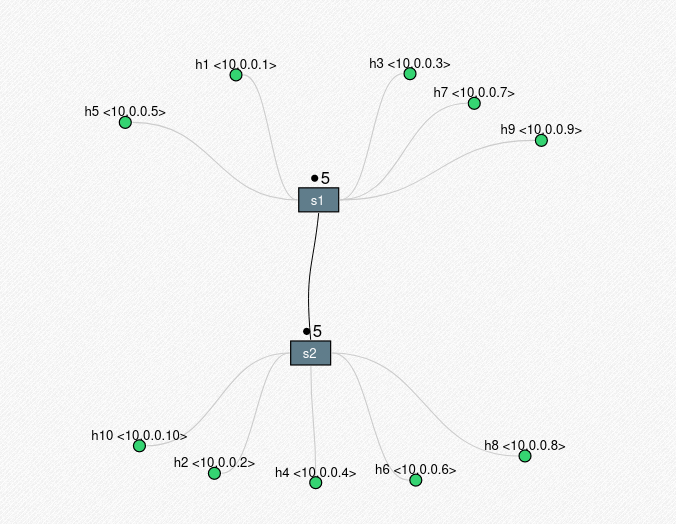
\includegraphics[width=0.9\linewidth]{images/mininet_topo.png}
    \caption{The resulting Dumbbell topology with the broker being h9 - the central node. The link between the central switch and the central host results in a congested network.}
    \label{fig:mininet-topo}
\end{figure}

Using the Python API provided, we created the network topology shown in Figure~\ref{fig:mininet-topo}.
The script takes several parameters to create the following three scenarios:

\begin{itemize}
    \item A synthetic scenario testing the limits of implementations.
    \item A realistic scenario based on a smart-home use-case.
    \item A realistic scenario based on a 3D printer farm.
\end{itemize}

The topology for all three scenarios remains the same - a minimum spanning tree of a typical IoT mesh network.
When designing this topology, we needed it to reflect various realistic IoT scenarios.
We can imagine this as a singular room in a home with all of its smart appliances being a cluster in the smart home or a cluster of 3D printers in a section of a farm in the 3D printer farm.
The critical feature of this topology is that many clusters are connected to a central broker that controls the topology, hence creating a dumbbell structure.
The full definition of this topology can be found in Appendix~\ref{appendix:topo}.
The variables that the script changes between scenarios and simulations are the link's \textit{bandwidth}, \textit{delay} and the rate of \textit{packet loss}.

The bandwidth of a link is the maximum rate of data transfer we can achieve.
In contrast to bandwidth in signal processing, we measure bandwidth in bits per second rather than hertz in computer networking.
The delay of a link specifies the latency of the link.
It is the time that a bit of data takes to travel across a link. 
We measure this in milliseconds.
Link delay corresponds to the geographical distance between the communicating parties; however, in the case of IoT, we can expect devices to be in local proximity.
Lastly, the packet loss rate shows the percentage of corrupted or dropped packets in transit.
Various protocols having to retransmit packets also adds to the delay of data transfer.
Importantly, we have only considered the typical circumstances of packet loss and have not included scenarios such as interference or packet loss attacks.

The bandwidth and delay numbers correspond, as closely as possible, to various link types in a network.
To do so, for the smart-home scenario, we have gathered data from the~\cite{ofcom_uk_2021} report on UK broadband speeds.
There were specific cases in which it was not possible to find this data in the report; hence it was augmented using a similar methodology in work conducted by~\cite{previdi_is-is_2019} and in the case of ZigBee, the work by~\citet{alena_fault_2011}.

\begin{table}[ht]
    \caption{The parameters chosen for each link simulation in Mininet in the smart home scenario. The types of links were chosen as the most commonly occurring ones in IoT use cases.}\label{tab:links:home}
    %\tt 
    \rowcolors{2}{}{gray!3}
    \begin{tabular}{@{}llll@{}}
        \toprule
        \textbf{Simulated Link Type} & \textbf{Link bandwidth (Mb/s)} & \textbf{Link delay (ms)} & \textbf{Packet loss rate (\%)} \\
        Wi-Fi                        & \texttt{30}                    & \texttt{10}              & \texttt{2}                     \\
        ZigBee                       & \texttt{0.25}                  & \texttt{5}               & \texttt{1}                     \\
        4G                           & \texttt{4}                     & \texttt{20}              & \texttt{1.5}                   \\
        3G                           & \texttt{1}                     & \texttt{40}              & \texttt{1.5}                   \\
        100Mb Ethernet               & \texttt{100}                   & \texttt{1}               & \texttt{0.2}                   \\
        \bottomrule
    \end{tabular}
\end{table}

Hence, we expect that the bandwidth and link delay numbers accurately represent a real-world scenario.
However, it was complicated to find exact estimates for packet loss rates, with most sources describing approximations for a stable connection~\citep{sdu_ictp-sdu_2013} and not precise measurements.
Hence, the data are best estimates, cross-validated through the different sources and are not exact values.

In the case of the smart home scenario, as presented in Table~\ref{tab:links:home}, we expect that our packet loss rates are accurate as these, as previously stated, do appear in the home broadband reports and other studies.
In the case of the 3D printer, as presented in Table~\ref{tab:links:3d} farm scenario, due to the number of machines and the interference these cause in a 3D printer farm, we modelled this scenario to have more packet loss.
We specifically chose this scenario to test the benefits that QUIC should receive in an environment with high packet loss.
However, we found it difficult to find exact data on packet loss percentages in smart factories or workshops; hence, we expect a margin of error on some of the values.

In general, we can assume that the packet loss rates will increase by some constant factor across all links.
Hence, we have also created a synthetic scenario with extreme packet loss as presented in Table~\ref{tab:links:synth}.
If the protocol performs well for an extreme scenario, we can expect it to also perform well for packet loss percentages up to that scenario.

\begin{table}[ht]
    \caption{The parameters chosen for each link simulation in Mininet in the 3D printer farm scenario. The data assumes a typical IoT setup where most devices are within local geographical proximity. That is, the devices are communicating with each other within the range of one factory or site, with only the central node communicating with some server.}\label{tab:links:3d}
    %\tt 
    \rowcolors{2}{}{gray!3}
    \begin{tabular}{@{}llll@{}}
        \toprule
        \textbf{Simulated Link Type} & \textbf{Link bandwidth (Mb/s)} & \textbf{Link delay (ms)} & \textbf{Packet loss rate (\%)} \\
        Wi-Fi                        & \texttt{30}                    & \texttt{10}              & \texttt{5}                     \\
        ZigBee                       & \texttt{0.25}                  & \texttt{5}               & \texttt{3}                     \\
        4G                           & \texttt{4}                     & \texttt{20}              & \texttt{2.5}                   \\
        3G                           & \texttt{1}                     & \texttt{40}              & \texttt{2.5}                   \\
        100Mb Ethernet               & \texttt{100}                   & \texttt{1}               & \texttt{0.5}                   \\
        \bottomrule
    \end{tabular}
\end{table}

\begin{table}[ht]
    \caption{The parameters chosen for each link simulation in Mininet in the synthetic scenario. Here we opt for extreme packet loss scenarios to test the boundaries of the protocols. We opted for 20 times the normal packet loss that the link can expect in each case. We have also tested this for higher values however all protocol implementations greatly suffered in performance beyond this.}\label{tab:links:synth}
    %\tt 
    \rowcolors{2}{}{gray!3}
    \begin{tabular}{@{}llll@{}}
        \toprule
        \textbf{Simulated Link Type} & \textbf{Link bandwidth (Mb/s)} & \textbf{Link delay (ms)} & \textbf{Packet loss rate (\%)} \\
        Wi-Fi                        & \texttt{30}                    & \texttt{10}              & \texttt{15}                     \\
        ZigBee                       & \texttt{0.25}                  & \texttt{5}               & \texttt{15}                     \\
        4G                           & \texttt{4}                     & \texttt{20}              & \texttt{20}                   \\
        3G                           & \texttt{1}                     & \texttt{40}              & \texttt{20}                   \\
        100Mb Ethernet               & \texttt{100}                   & \texttt{1}               & \texttt{4}                   \\
        \bottomrule
    \end{tabular}
\end{table}

We evaluate MQuicTT's performance using the presented topologies and respective simulation parameters in the following way.
Each protocol transmits 100 messages from a client to a broker for each data link.

During this, we measure the following:

\begin{itemize}
    \item The time taken for the underlying transport protocol to establish a connection.
    \item The time taken to transmit the message to the broker.
\end{itemize}

This is repeated several times to ensure that variance does not affect results.
This process is repeated for all three testing scenarios.

In general, MQTT allows for messages with a maximum size of approximately 260MB.
However, this is a huge message, and most publicly deployed brokers reject it, so we created a representative message for each use case.
Each topic in MQTT consists of a hierarchy of topic levels separated by a forward slash.
For example, in a smart home scenario, we may have a topic like $home/groundfloor/kitchen/temp$ to control the temperature in the kitchen via a smart thermostat.
A topic may also include a wildcard.
The topic string $home/groundfloor/+/temp$ includes a \textit{single-level} wildcard that will match an arbitrary string.
This would match the topic $home/groundfloor/lounge/temp$, but not match the topic $home/secondfloor/kitchen/temp$.
If a client wishes to subscribe to multiple topics with the same prefix, a \textit{multi-level} wildcard may be used.
For example, the topic $home/secondfloor/kitchen/\#$ can be used to subscribe to all topics with a prefix matching the string before the hash character.
Notably, brokers reserve topics for system messages starting with the \$ character.

The chosen topic and the transmitted message for each scenario can be found in Appendix~\ref{appendix:mqtt_message}.
The messages were devised based on an arbitrary command that may be issued to an IoT device present in the scenario.
For the synthetic scenario we opted to use a message that is considerably longer, to test the limits of each implementation.
This message simply consisted of a paylaod with a field replicated thousands of times.
It has ben omitted from the Appendix due to being too long.
\chapter{Analysis} \label{chapter:eval}

This section presents the analysis results conducted using the previously described methodology.
The analysis is broadly split into two stages: performance analysis and binary size analysis.
The experiment design for the performance analysis can be found in Section~\ref{chap:net_sim}, and the experiment design for the binary analysis can be found in Section~\ref{sec:exp_bin}.
The performance analysis is further split into a connection time analysis and a general transmission time analysis.

\section{Network performance experiment design} \label{chap:net_sim}

We now discuss the analysis methodology for the performance portion of the implementation evaluation.
That is, this section focuses on evaluating MQuicTT against the base $rumqtt$ implementation.

The critical consideration for this design is the scenarios in which IoT devices are used.
When evaluating the network performance of the implementations, we considered two options: using real IoT devices or using a network simulation tool.
Due to technical limitations that came with using real devices, such as not being able to access the router of our network, we opted for simulation.
In this section, we will discuss how we used Mininet~\citep{lantz_mininet_2021}, a realistic virtual network, in our evaluation.

Mininet is a tool that network developers and researchers can use to create software-defined networks (SNDs) using the $OpenFlow$ standard.

\begin{figure}[ht]
    \centering
    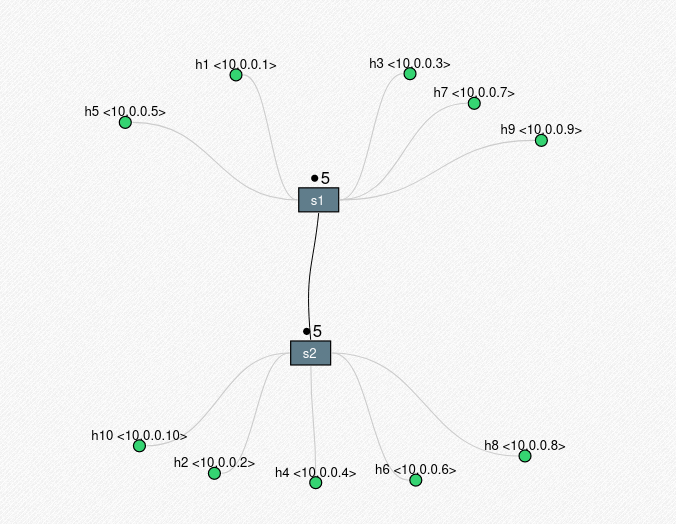
\includegraphics[width=0.9\linewidth]{images/mininet_topo.png}
    \caption{The resulting Dumbbell topology with the broker being h9 - the central node. The link between the central switch and the central host results in a congested network.}
    \label{fig:mininet-topo}
\end{figure}

Using the Python API provided, we created the network topology shown in Figure~\ref{fig:mininet-topo}.
The script takes several parameters to create the following three scenarios:

\begin{itemize}
    \item A synthetic scenario testing the limits of implementations.
    \item A realistic scenario based on a smart-home use-case.
    \item A realistic scenario based on a 3D printer farm.
\end{itemize}

The topology for all three scenarios remains the same - a minimum spanning tree of a typical IoT mesh network.
When designing this topology, we needed it to reflect various realistic IoT scenarios.
We can imagine this as a singular room in a home with all of its smart appliances being a cluster in the smart home or a cluster of 3D printers in a section of a farm in the 3D printer farm.
The critical feature of this topology is that many clusters are connected to a central broker that controls the topology, hence creating a dumbbell structure.
The full definition of this topology can be found in Appendix~\ref{appendix:topo}.
The variables that the script changes between scenarios and simulations are the link's \textit{bandwidth}, \textit{delay} and the rate of \textit{packet loss}.

The bandwidth of a link is the maximum rate of data transfer we can achieve.
In contrast to bandwidth in signal processing, we measure bandwidth in bits per second rather than hertz in computer networking.
The delay of a link specifies the latency of the link.
It is the time that a bit of data takes to travel across a link. 
We measure this in milliseconds.
Link delay corresponds to the geographical distance between the communicating parties; however, in the case of IoT, we can expect devices to be in local proximity.
Lastly, the packet loss rate shows the percentage of corrupted or dropped packets in transit.
Various protocols having to retransmit packets also adds to the delay of data transfer.
Importantly, we have only considered the typical circumstances of packet loss and have not included scenarios such as interference or packet loss attacks.

The bandwidth and delay numbers correspond, as closely as possible, to various link types in a network.
To do so, for the smart-home scenario, we have gathered data from the~\cite{ofcom_uk_2021} report on UK broadband speeds.
There were specific cases in which it was not possible to find this data in the report; hence it was augmented using a similar methodology in work conducted by~\cite{previdi_is-is_2019} and in the case of ZigBee, the work by~\citet{alena_fault_2011}.

\begin{table}[ht]
    \caption{The parameters chosen for each link simulation in Mininet in the smart home scenario. The types of links were chosen as the most commonly occurring ones in IoT use cases.}\label{tab:links:home}
    %\tt 
    \rowcolors{2}{}{gray!3}
    \begin{tabular}{@{}llll@{}}
        \toprule
        \textbf{Simulated Link Type} & \textbf{Link bandwidth (Mb/s)} & \textbf{Link delay (ms)} & \textbf{Packet loss rate (\%)} \\
        Wi-Fi                        & \texttt{30}                    & \texttt{10}              & \texttt{2}                     \\
        ZigBee                       & \texttt{0.25}                  & \texttt{5}               & \texttt{1}                     \\
        4G                           & \texttt{4}                     & \texttt{20}              & \texttt{1.5}                   \\
        3G                           & \texttt{1}                     & \texttt{40}              & \texttt{1.5}                   \\
        100Mb Ethernet               & \texttt{100}                   & \texttt{1}               & \texttt{0.2}                   \\
        \bottomrule
    \end{tabular}
\end{table}

Hence, we expect that the bandwidth and link delay numbers accurately represent a real-world scenario.
However, it was complicated to find exact estimates for packet loss rates, with most sources describing approximations for a stable connection~\citep{sdu_ictp-sdu_2013} and not precise measurements.
Hence, the data are best estimates, cross-validated through the different sources and are not exact values.

In the case of the smart home scenario, as presented in Table~\ref{tab:links:home}, we expect that our packet loss rates are accurate as these, as previously stated, do appear in the home broadband reports and other studies.
In the case of the 3D printer, as presented in Table~\ref{tab:links:3d} farm scenario, due to the number of machines and the interference these cause in a 3D printer farm, we modelled this scenario to have more packet loss.
We specifically chose this scenario to test the benefits that QUIC should receive in an environment with high packet loss.
However, we found it difficult to find exact data on packet loss percentages in smart factories or workshops; hence, we expect a margin of error on some of the values.

In general, we can assume that the packet loss rates will increase by some constant factor across all links.
Hence, we have also created a synthetic scenario with extreme packet loss as presented in Table~\ref{tab:links:synth}.
If the protocol performs well for an extreme scenario, we can expect it to also perform well for packet loss percentages up to that scenario.

\begin{table}[ht]
    \caption{The parameters chosen for each link simulation in Mininet in the 3D printer farm scenario. The data assumes a typical IoT setup where most devices are within local geographical proximity. That is, the devices are communicating with each other within the range of one factory or site, with only the central node communicating with some server.}\label{tab:links:3d}
    %\tt 
    \rowcolors{2}{}{gray!3}
    \begin{tabular}{@{}llll@{}}
        \toprule
        \textbf{Simulated Link Type} & \textbf{Link bandwidth (Mb/s)} & \textbf{Link delay (ms)} & \textbf{Packet loss rate (\%)} \\
        Wi-Fi                        & \texttt{30}                    & \texttt{10}              & \texttt{5}                     \\
        ZigBee                       & \texttt{0.25}                  & \texttt{5}               & \texttt{3}                     \\
        4G                           & \texttt{4}                     & \texttt{20}              & \texttt{2.5}                   \\
        3G                           & \texttt{1}                     & \texttt{40}              & \texttt{2.5}                   \\
        100Mb Ethernet               & \texttt{100}                   & \texttt{1}               & \texttt{0.5}                   \\
        \bottomrule
    \end{tabular}
\end{table}

\begin{table}[ht]
    \caption{The parameters chosen for each link simulation in Mininet in the synthetic scenario. Here we opt for extreme packet loss scenarios to test the boundaries of the protocols. We opted for 20 times the normal packet loss that the link can expect in each case. We have also tested this for higher values however all protocol implementations greatly suffered in performance beyond this.}\label{tab:links:synth}
    %\tt 
    \rowcolors{2}{}{gray!3}
    \begin{tabular}{@{}llll@{}}
        \toprule
        \textbf{Simulated Link Type} & \textbf{Link bandwidth (Mb/s)} & \textbf{Link delay (ms)} & \textbf{Packet loss rate (\%)} \\
        Wi-Fi                        & \texttt{30}                    & \texttt{10}              & \texttt{15}                     \\
        ZigBee                       & \texttt{0.25}                  & \texttt{5}               & \texttt{15}                     \\
        4G                           & \texttt{4}                     & \texttt{20}              & \texttt{20}                   \\
        3G                           & \texttt{1}                     & \texttt{40}              & \texttt{20}                   \\
        100Mb Ethernet               & \texttt{100}                   & \texttt{1}               & \texttt{4}                   \\
        \bottomrule
    \end{tabular}
\end{table}

We evaluate MQuicTT's performance using the presented topologies and respective simulation parameters in the following way.
Each protocol transmits 100 messages from a client to a broker for each data link.

During this, we measure the following:

\begin{itemize}
    \item The time taken for the underlying transport protocol to establish a connection.
    \item The time taken to transmit the message to the broker.
\end{itemize}

This is repeated several times to ensure that variance does not affect results.
This process is repeated for all three testing scenarios.

In general, MQTT allows for messages with a maximum size of approximately 260MB.
However, this is a huge message, and most publicly deployed brokers reject it, so we created a representative message for each use case.
Each topic in MQTT consists of a hierarchy of topic levels separated by a forward slash.
For example, in a smart home scenario, we may have a topic like $home/groundfloor/kitchen/temp$ to control the temperature in the kitchen via a smart thermostat.
A topic may also include a wildcard.
The topic string $home/groundfloor/+/temp$ includes a \textit{single-level} wildcard that will match an arbitrary string.
This would match the topic $home/groundfloor/lounge/temp$, but not match the topic $home/secondfloor/kitchen/temp$.
If a client wishes to subscribe to multiple topics with the same prefix, a \textit{multi-level} wildcard may be used.
For example, the topic $home/secondfloor/kitchen/\#$ can be used to subscribe to all topics with a prefix matching the string before the hash character.
Notably, brokers reserve topics for system messages starting with the \$ character.

The chosen topic and the transmitted message for each scenario can be found in Appendix~\ref{appendix:mqtt_message}.
The messages were devised based on an arbitrary command that may be issued to an IoT device present in the scenario.
For the synthetic scenario we opted to use a message that is considerably longer, to test the limits of each implementation.
This message simply consisted of a paylaod with a field replicated thousands of times.
It has ben omitted from the Appendix due to being too long.
\section{Connection time comparison} \label{sec:conn_time}

In this section of the analysis, we focus on connection time.
By connection time, we mean two things: the time it takes for the underlying transport protocol to establish a secure connection and the total time taken before MQTT sends its first data packet.

Connection time is essential in IoT devices as many do not connect while idling.
A device may opt not to be connected at all times to reduce energy consumption and computational power.
The device will then establish a connection and transmit data whenever required.
However, this means that some efficiency is lost if the connection has to be constantly re-established.
Hence, MQTT defines the period to keep the connection alive as the \textit{keep alive interval}.
In an MQTT/TCP implementation, the standard way to extend the keep alive interval is to periodically send a $ping$ packet, forcing the connection to remain open.
However, it has been shown that this method can lead to security vulnerabilities~\citep{vaccari_slowtt_2020,mileva_comprehensive_2021}.

We have talked previously about QUIC having a less complex handshake and hence being able to establish a secure connection quicker than TCP/TLS.
Hence, using QUIC in MQTT is a step closer to providing the needed efficiency while not having to use methods that may lead to vulnerabilities.

To measure the connection time we have began a communication via MQuicTT and the other MQTT implementations and captured it using $tcpdump$.
We have then extracted the time between the start of the QUIC or TCP communication and the completion of the handshake, as well as the time before MQTT sends its first data packet.
The results of this are shown in Figure TBA.

[Figure here]

[Discussion here]
\section{Data transmission comparison}

We next evaluate the time it took both implementations to transmit the aforementioned MQTT messages.
To do so, we have used the previously described methodology.
That is, we have transmitted the MQTT messages shown in~\ref{appendix:mqtt_message} for their respective scenario and have measured the total time taken for the transmission to occur.
We have repeated this and taken the average of the results to ensure that they are representative.

Based on the analysis of connection time and previous discussions, we hypothesise that:

\begin{itemize}
    \item \textbf{H1}: $MQuicTT$ performs on-par with $rumqtt$ in the IoT home scenario but does not present a significant difference.
    \item \textbf{H2}: $MQuicTT$ performs significantly better than $rumqtt$ in the printer farm scenario.
    \item \textbf{H3}: $MQuicTT$ can transmit all the messages on all data links in the synthetic scenario, whereas $rumqtt$ is not.
\end{itemize}

Figure~\ref{fig:comm_time} shows the results of this experiment.

We can see that the results support hypothesis \textbf{H1}.
That is,  $MQuicTT$ performs almost identically to $rumqtt$ across all data links for the IoT home scenario.
In fact, $MQuicTT$ actually performs marginally better than $rumqtt$ in this scenario with the transmission time of $MQuicTT$ being on average $2.02\%$ lower than that of $rumqtt$.
From this we can see that $MQuicTT$ presents no disadvantages in terms of transmission time even in network with low packet loss and congestion.
For new deployments it would be advantages to use $MQuicTT$, however, for existing ones, it may not be advisable to migrate deployments.

Hypothesis \textbf{H2} however is not supported.
The performance advantage in terms of transmission time for $MQuicTT$ in the printer farm scenario is almost identical to that of the smart home scenario.
On average, $MQuicTT$ transmits the data $2.36\%$ faster than $rumqtt$ and although this is an improvement, it is comparable to the improvement in the IoT home scenario.
Hence, the results draw a similar conclusion to that of the IoT home scenario.
It is still advantages to use $MQuicTT$ for new deployments.

The results of the printer farm scenario show that the presented use-case does not present a high enough packet loss percentage for $MQuicTT$ to have a significant advantage.
This can be verified by looking at the synthetic scenario, which validates hypothesis \textbf{H3}.
In the synthetic scenario only $MQuicTT$ managed to transmit the data on all data links and transmitted the data $13.8\%$ faster using ethernet.
Hence, in environments that may experience extreme data loss, $MQuicTT$ presents a clear advantage, however, finding such a scenario may be difficult.

Overall, $MQuicTT$ transmitted the data faster than $rumqtt$ across all scenarios and has shown to be more resilient against high packet loss.
It may however be ineffective overhead to migrate existing deployments to it due to the marginal benefits in low congestion environments.

\section{Binary size experiment design} \label{sec:exp_bin}

The last section of this chapter describes how we have conducted further analysis on the binary size of the QUIC protocol that underlines MQuicTT.
The focus of this section is to see if the QUIC stack contributes a significant overhead to MQuicTT's binary size and how we can reduce this overhead.
We expect that the QUIC stack will contribute to the majority of the size of MQuicTT as MQTT itself is designed to have a low code size overhead.
Hence, the first step of this part of the analysis will be to determine how much QUIC contributes to the binary size.

In order to get a breakdown of the binary we have used the $cargo-bloat$~\footnote{cargo-bloat - \url{https://lib.rs/crates/cargo-bloat}} utility.
The utility analyses the binary using custom ELF, DWARF and Mach-O parsers and disassembles the binary to look for references and links to anonymous data.
Doing so creates a map of the binary that shows where every byte has a label attached to it.

This utility provides the composition of a Rust binary. 
However, it is not perfect and results in some margin of error.
Unfortunately, this margin of error is also not easily measurable.
By comparing the total size of the binary as reported by $cargo-bloat$ to the size reported by the operating system, we have deduced that the total error margin is within $1\%$ with good precision.
This should mean that we can get a somewhat accurate error margin on the components. 
However, it is also possible that the internal calculations are inaccurate despite the overall size being accurate.

The next step in this stage will be analysing methods for trimming down the QUIC stack binary size.
Hence, in this stage, we shift our focus to the binary produced by $QuicSocket$.
To reduce the binary size, we opt to use the method established by~\citet{eggert_towards_2020} as recreating these steps may show a general framework for reducing binary sizes for hardware constrained devices.
Notably, our application already handles client and server code separately; the MQTT broker requires a different binary to the MQTT client.

Hence, the steps we take are as follows:

\begin{itemize}
    \item Compile the binary for a 32-bit target by setting the $target$ flag in cargo to $i686-unknown-linux-gnu$.
    \item Remove any error handling code beyond what is needed for the binary to compile.
    \item Remove any code that writes to standard output.
\end{itemize}

After every step, we record the difference in binary size made by the change using the same methodology.

Once this step is completed we further analyse the size of $Quinn$ and $Rustls$ using a by-function binary size breakdown.
Using the $cargo-bloat$ utility we can get a list of the contribution of each function to the binary size and then assign each function to its respective protocol feature.

\section{Binary size breakdown} \label{sec:binary_sizes}

We first look at an in-depth breakdown of the composition of the binary of the underlying QUIC implementation.
As previously established, hardware constrained devices do not have much space for firmware; hence, identifying sections of the QUIC stack that can be trimmed down or eliminated entirely is essential.
In order to get a breakdown of the binary we have used the $cargo-bloat$~\footnote{cargo-bloat - \url{https://lib.rs/crates/cargo-bloat}} utility.

[figure of results here]

[discussion of results here]

In order to reduce the binary size we opt to use the method established by~\citet{eggert_towards_2020} as recreating these steps may show a general framework for reducing binary sizes for hardware constrained devices.
Notably, our application already handles client and server code separately; the MQTT broker requires a different binary to the MQTT client.

Hence, the steps we have taken are as follows:

\begin{itemize}
    \item Compile the binary for a 32-bit target by setting the $target$ flag in cargo to $i686-unknown-linux-gnu$.
    \item Remove any error handling code beyond what is needed for the binary to compile.
    \item Remove any code that writes to standard output.
\end{itemize}

The resulting binary sizes after these steps can be found in Figure TBA.

[Figure here]

As we can see, after trimming down the binary, the TLS implementation stands out as the most considerable dependency.
While~\cite{eggert_towards_2020} attempts to address this by creating minimal cypher implementations used by TLS, we instead opt to discuss the possibility of a complete alternative to TLS, suitable for hardware constrained devices in Section~\ref{chap:TLS}.


\subsection{Summary}

When discussing the possibility of using a Rust QUIC implementation as the transport layer protocol for network firmware in IoT devices we established that the QUIC implementation must perform at least as well as the baseline and have a binary size which can fit onto widely used IoT devices.

From the above analysis we can conclude that $MQuicTT$ performs at least as well as the baseline TCP implementation of $rumqtt$.
When it comes to connection time, $MQuicTT$ performs marginally better, and when it comes to total transmission time, the implementations are on par.
Hence, this requirement is satisfied.

In terms of binary size we have managed to reduce it to approximately $8Mb$.
This size of binary would easily be installable on popular IoT devices such as the Raspberry Pi 3 Model B, Beagle Board or the Arduino Due.
However, this size of binary would not support industrially-wide used chips such as the esp32.
We have analysed the possible avenues of further reducing the binary size of $MQuicTT$ by addressing issues with the regex library and by analysing $Quinn$ and $Rustls$ by feature.
Hence, overall, we can say that we have achieved creating an implementation that can be used on a large number of IoT devices, but not on ones with stricter hardware constraints.

\chapter{Conclusion} \label{chap:conclusion}
\begin{appendices}
    \chapter{Data}
    \chapter{MQTT simulation messages}\label{appendix:mqtt_message}

\begin{lstlisting}[caption = {The message payload and topic used to transmit for the printer farm scenario.}, label={lst:msg_farm}]
Topic
------

GENERICO-CORPO/JSON/0/1/ADDITIVE-MANUFACTURING-13/PRINT/1

Payload
-------

"print" = {
    "Timestamp"="20201001 171035",
    "BedTemp"="75",
    "ExtruderTemp"="205",
    "Adhesion"="Skirt",
    "File"="/home/prints/part.gcode",
    "Speed"="50 mm/s",
    "Layer Height"="0.12 mm",
    "Retraction"="6mm at 25mm/s",
    "Infill"="20%",
    "Initial layer speed"="20 mm/s",
    "Initial fan speed"="0%"
}
\end{lstlisting}

\begin{lstlisting}[caption = {The message payload and topic used to transmit for the printer home scenario.}, label={lst:msg_home}]
Topic
------

HOME/JSON/0/1/SET-TEMP

Payload
-------

"req" = {
    "Room"="Bedroom",
    "Device"="AC",
    "Temp"="17",
}
\end{lstlisting}
\end{appendices}
\bibliographystyle{abbrvnat}
\bibliography{l4proj}
\end{document}
